% Results under circuit-level SI1000 and SD6 noise (sdim 1.4.0 runs, 2026-10), Secs. 3.1 to 3.5 (track sim).
% Rewritten 2026-11-13 with the journal-paper-writing skill (PLAN Sec. 2; CONTRACT Secs. 3 to 5 and 9).
% Every number is checked against the data by paper-rework/jpw-review/sim/check_numbers.py (prose numbers:
% checks_prose.py, ids in the comments below; table bodies between "BEGIN GEN" and "END GEN" are generated
% by "check_numbers.py --write" and must not be edited by hand).
% Outline and sentence tables: paper-rework/jpw-review/sim/results-outline.md, results-sentence-tables.md.

% Scope sentence of the section (facts that the Methods leave to the Results, hand-off M1, Sec. 2).
Unless stated otherwise, the results are for the one-ancilla layout and come from the production runs; the pseudo-thresholds also use the high-$p$ extension runs (\autoref{tab:runs}). We write $r_{\mathrm{LRB}}$ and $r_{\mathrm{RB}}$ for the fitted error rates per unit of depth of LRB-D and of the baseline. We analyze the intervals $k = 1$ to $4$; for larger intervals the accepted decay departs further from a single exponential (\autoref{tab:chi_largek}, for $p = 5\times10^{-3}$).

\subsection{Terminal Postselection}
\label{sub:terminal_results}

% checks T-def-*, T-fac-*, T-p-double, T-sd6-fac (facts/raw_per_depth.csv, schedule const-0)
Under terminal postselection the accepted logical signal does not decay as a single exponential (\autoref{fig:const0_si1000_1anc}). The traces stay flat at small depth and then bend down: the deficit $1 - \langle \bar{X} \rangle$, while it is small, grows about quadratically in the depth and in $p$. Under SI1000 at $p = 10^{-3}$ it grows from $1.7\times10^{-5}$ at $m = 2$ to $2.0\times10^{-3}$ at $m = 22$, by a factor of 119 where a quadratic law gives 121, while the deficit $1 - \langle Z \rangle$ of the baseline grows by a factor of 10, where a linear law gives 11. At $m = 10$, doubling $p$ from $5\times10^{-4}$ to $10^{-3}$ multiplies the deficit by 4.0. Under SD6 the deficit grows by a factor of 28 from $m = 2$ to $10$ at $p = 10^{-3}$, where a quadratic law gives 25 (\autoref{fig:const0_sd6_1anc}). These circuits are noiseless at $m = 0$, where $\langle \bar{X} \rangle = 1$, so a single exponential would give a deficit that is linear in $m$ at small depth. We therefore extract no error rate from terminal postselection.

\begin{figure*}[tp]
  \centering
  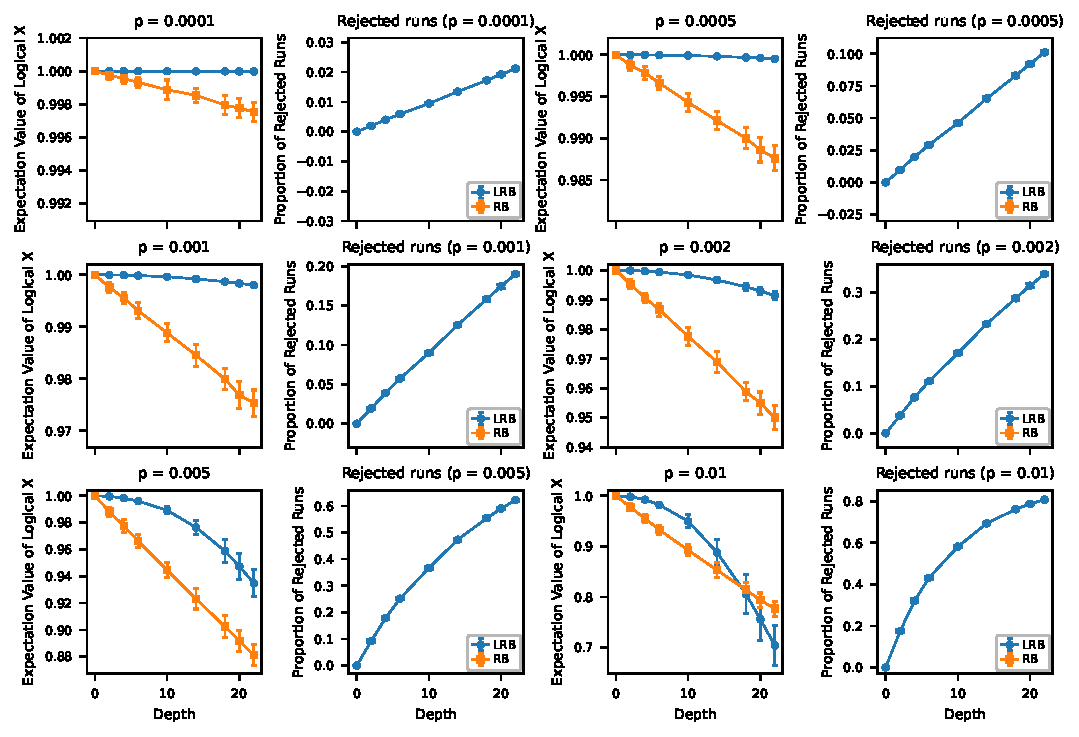
\includegraphics[width=0.95\textwidth]{figures/sdim140/si1000-1anc-const-0-nofit.pdf}
  \caption{Terminal postselection under SI1000, from the run of the one-ancilla layout, at the two-qutrit gate error probabilities $p = 10^{-4}$, $5\times10^{-4}$, $10^{-3}$, $2\times10^{-3}$, $5\times10^{-3}$ and $10^{-2}$. In each pair of panels, the left panel shows the accepted logical signal $\langle \bar{X} \rangle$ of LRB-D (blue) and the physical signal $\langle Z \rangle$ of physical RB at the same $p$ (orange) versus the depth $m$, and the right panel shows the fraction of rejected LRB-D shots; the baseline rejects none. In the figure, ``LRB'' stands for LRB-D, ``Rejected Runs'' for rejected shots, and the axis label ``Expectation Value of Logical X'' marks the signal of both curves. Error bars are standard deviations over the 30 sequences for the signals and standard errors over the sequences for the rejected fraction. The legend in each right panel labels the curves of the left panel. No fits are drawn.}
  \label{fig:const0_si1000_1anc}
\end{figure*}

% checks T-budget-*, T-model-* (raw_per_depth.csv, schedule const-0; fault counts: jpw-review/hw/checks/check_fault_budgets.out)
The quadratic growth of the deficit is that of pairs of faults. Growth as $p^2$ means that, to leading order, an accepted shot with a wrong logical outcome carries two faults, and the number of pairs of fault locations grows as $m^2$. A single fault cannot produce such a shot: the logical Cliffords keep it on one qutrit or on the pair $q_2$, $q_3$, and there it shifts the logical outcome only through a $Z$ component on $q_0$ or $q_3$, which also shifts the value of $G_3$ or $G_4$. A logical Clifford puts five times as many expected faults on the data qutrits under SD6 as under SI1000 (\autoref{sub:noise_models}), so pairs of faults predict a deficit about 25 times larger, if a pair escapes equally often under both models. At $p = 10^{-3}$ the deficit under SD6 is 32 times larger at $m = 22$, where it has reached $6.3\times10^{-2}$ and higher orders enter, and 23 to 25 times larger at the depths $m \le 6$.

% checks T-rej-*, T-sat, T-sig-sat (raw_per_depth.csv); grid points where the signal falls below the baseline: generated table const0, checks T-below-*
At large depth and $p$ terminal postselection brings no gain: it rejects most shots, and the accepted logical signal falls below the physical signal. Under SI1000 at $p = 5\times10^{-3}$ the rejected fraction is 9.2\% at $m = 2$, 37\% at $m = 10$ and 62\% at $m = 22$. The rejected fraction saturates at $8/9$, the value for uniformly random outcomes of the two $X$-type stabilizers, of whose nine joint values one is accepted; under SD6 it is $0.8889$ at $p = 10^{-2}$ and $m = 22$ (\autoref{fig:const0_sd6_1anc}). Because the deficit of LRB-D grows faster with $p$ than that of the baseline, $\langle \bar{X} \rangle$ falls below $\langle Z \rangle$ as $p$ grows, at $m = 22$ between $p = 7.5\times10^{-3}$ and $10^{-2}$ under SI1000 and between $2\times10^{-3}$ and $5\times10^{-3}$ under SD6 (\autoref{tab:const0}, which also gives $m = 10$).

% checks T-2anc-* (raw_per_depth.csv, configs conv-*); grid points: generated table const0
The run of the two-ancilla layout, whose circuits for terminal postselection are built in the same way from 30 newly drawn sequences (\autoref{sub:sim_framework}), reproduces the traces of \autoref{fig:const0_si1000_1anc} and \autoref{fig:const0_sd6_1anc} for $p$ from $10^{-3}$ to $10^{-2}$: no deficit differs between the two runs by more than two standard errors over the sequences. At $m = 10$ and $22$, its deficits agree with those of the one-ancilla run within 3\% under SI1000 and 6\% under SD6, and its rejected fractions within $0.6$ percentage points. At $m \le 6$, where the deficits are small, they differ by up to 16\%, and the deficit under SD6 at $p = 10^{-3}$ is 27 to 29 times that under SI1000. At $m = 10$ and $22$ the accepted logical signal of this run first falls below $\langle Z \rangle$ at the same grid points as in the one-ancilla run (\autoref{tab:const0}, \autoref{fig:const0_si1000_2anc}, \autoref{fig:const0_sd6_2anc}).

\subsection{Postselection on Every Check Round}
\label{sub:interval_results}

% checks K1-ratio-*, K1-exp-* (facts/fits_all_k.csv, k = 1); table body: generated table k1
With every check round postselected ($k = 1$), the fitted logical error rate per unit of depth at $p = 10^{-3}$ is smaller than that of the baseline by a factor of $92(9)$ under SI1000 and $96(2)$ under SD6, where the parentheses give the standard deviation of the parametric bootstrap (\autoref{tab:k1_error_rates}). The advantage shrinks as $p$ grows, to factors of 2.1 and 4.3 at $p = 2\times10^{-2}$, because the two error rates scale differently. Between $p = 5\times10^{-4}$ and $2\times10^{-3}$, $r_{\mathrm{LRB}}$ grows as $p^{2.0}$ under SI1000 and as $p^{1.9}$ under SD6, with uncertainties of $0.2$ and $0.03$ in the exponents, and $r_{\mathrm{RB}}$ as $p^{1.0}$ under both (\autoref{fig:four_configs} in \autoref{sub:layout_comparison} shows both rates against $p$). From $2\times10^{-3}$ to $5\times10^{-3}$ the exponents are $2.1$ and $1.6$. From $p = 5\times10^{-3}$ to $2\times10^{-2}$, $r_{\mathrm{LRB}}$ grows faster than $p^2$ under both models: as $p^{2.4}$ and $p^{2.6}$ under SI1000 and as $p^{2.1}$ and $p^{2.4}$ under SD6 in the two steps of the grid. As under terminal postselection, a single fault in a logical Clifford stays on one qutrit or on the pair $q_2$, $q_3$; there the next check round detects it. Since a single fault in a check round never leads to a logical error that this round and the next both miss (\autoref{sub:ancilla_layouts}), the nearly quadratic growth at small $p$ is again that of pairs of faults.

\begin{table*}[tp]
  \centering
  \small
  \begin{tabular}{c|ccc|ccc}
    \hline
    & \multicolumn{3}{c|}{SI1000} & \multicolumn{3}{c}{SD6} \\
    $p$ & $r_{\mathrm{LRB}}$ & $r_{\mathrm{RB}}$ & $r_{\mathrm{RB}}/r_{\mathrm{LRB}}$ & $r_{\mathrm{LRB}}$ & $r_{\mathrm{RB}}$ & $r_{\mathrm{RB}}/r_{\mathrm{LRB}}$ \\
    \hline
    % BEGIN GEN k1
    $10^{-3}$ & $(8.3 \pm 0.8)\times10^{-6}$ & $7.6\times10^{-4}$ & $92 \pm 9$ & $(8.26 \pm 0.18)\times10^{-5}$ & $8.0\times10^{-3}$ & $96 \pm 2$ \\
    $5\times10^{-3}$ & $(2.27 \pm 0.12)\times10^{-4}$ & $3.8\times10^{-3}$ & $16.8 \pm 0.9$ & $(1.38 \pm 0.04)\times10^{-3}$ & $3.9\times10^{-2}$ & $28.1 \pm 0.8$ \\
    $10^{-2}$ & $(1.16 \pm 0.04)\times10^{-3}$ & $7.6\times10^{-3}$ & $6.6 \pm 0.2$ & $(6.05 \pm 0.20)\times10^{-3}$ & $7.6\times10^{-2}$ & $12.5 \pm 0.4$ \\
    $2\times10^{-2}$ & $(7.15 \pm 0.24)\times10^{-3}$ & $1.5\times10^{-2}$ & $2.10 \pm 0.07$ & $(3.29 \pm 0.21)\times10^{-2}$ & $1.4\times10^{-1}$ & $4.3 \pm 0.3$ \\
    % END GEN k1
    \hline
  \end{tabular}
  \caption{Fitted error rates per unit of depth in the one-ancilla layout, from the production runs, at four values of the two-qutrit gate error probability $p$: $r_{\mathrm{LRB}}$ for LRB-D with the postselection interval $k = 1$, $r_{\mathrm{RB}}$ for the baseline, physical RB under the same noise model at the same $p$, and their ratio. The uncertainties of $r_{\mathrm{LRB}}$ and of the ratio are standard deviations of the parametric bootstrap, which do not include the choice of sequences; that of $r_{\mathrm{RB}}$ is below 1\% of its value and is not shown. \autoref{tab:k1_depths} gives the number of depths in each fit.}
  \label{tab:k1_error_rates}
\end{table*}

% checks K1-rej-* (raw_per_depth.csv, schedule unif-1)
These error rates describe a fraction of the shots that shrinks with depth. Under SI1000 at $p = 5\times10^{-3}$ the postselection rejects 22\% of the shots at $m = 0$, 63\% at $m = 2$, 98.1\% at $m = 10$ and 99.98\% at $m = 22$, where about 200 of $10^6$ shots per sequence are accepted. The rejected fraction is smaller at smaller $p$, 55\% at $m = 10$ for $p = 10^{-3}$, and at $m = 10$ it is larger under SD6, 99.8\% for $p = 5\times10^{-3}$ (right panels of \autoref{fig:unif1_si1000_1anc} and \autoref{fig:unif1_sd6_1anc}).

\begin{figure*}[tp]
  \centering
  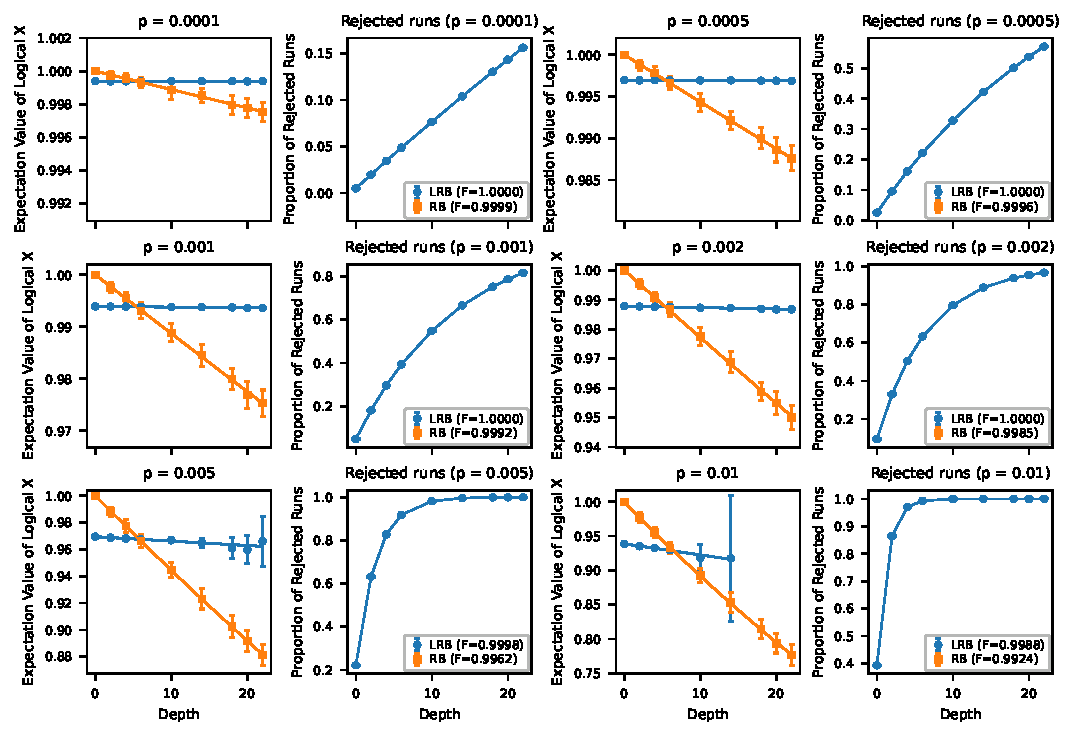
\includegraphics[width=0.95\textwidth]{figures/sdim140/si1000-1anc-unif-1-fit.pdf}
  \caption{Uniform-interval postselection with interval $k = 1$ under SI1000 in the one-ancilla layout, at the two-qutrit gate error probabilities $p = 10^{-4}$, $5\times10^{-4}$, $10^{-3}$, $2\times10^{-3}$, $5\times10^{-3}$ and $10^{-2}$. Left panels: accepted logical signal $\langle \bar{X} \rangle$ of LRB-D (blue; ``LRB'' in the legend) and physical signal $\langle Z \rangle$ of physical RB at the same $p$ (orange) versus the depth $m$, with the fits $F(m) = A f^m$ (lines); the axis label ``Expectation Value of Logical X'' marks the signal of both curves, and the legends in the right panels give the fitted average fidelity $\bar{F}$ per unit of depth as ``F''. Right panels: fraction of rejected LRB-D shots (``Rejected Runs''). Error bars are standard deviations over the 30 sequences for the signals and standard errors over the sequences for the rejected fraction. LRB-D points are missing at depths where a sequence has no accepted shot.}
  \label{fig:unif1_si1000_1anc}
\end{figure*}

% checks K1-chi-* (facts/fit_chi2.csv: lrb_chi2/(lrb_n_points - 2)), K1-slope-* (raw_per_depth.csv, 1anc-sd6)
The single exponential fitted for $r_{\mathrm{LRB}}$ describes the accepted decay approximately under SD6 and closely under SI1000 (\autoref{fig:unif1_si1000_1anc}, \autoref{fig:unif1_sd6_1anc}). Under SD6 the decay steepens with depth: at $p = 10^{-3}$ the signal drops by $6.6\times10^{-5}$ per unit of depth between $m = 0$ and $6$ and by $3.0\times10^{-4}$, 4.6 times as fast, between $m = 18$ and $22$. The steepening is consistent with the mirror inverse, in which no check round separates the Cliffords, so that pairs of faults accumulate as under terminal postselection, and with the larger expected number of faults of a logical Clifford under SD6. The SD6 values of $r_{\mathrm{LRB}}$, of the ratios of \autoref{tab:k1_error_rates} and of the exponents above are therefore effective values over the fitted depths, and their uncertainties do not include the dependence on these depths. Against the value $1/N_s = 0.03$ for residuals of the size of the standard errors (\autoref{sub:fit_model}), $\chi^2$ per degree of freedom for $10^{-3} \le p \le 10^{-2}$ is $0.5$ to $2.1$ under SD6 and $0.01$ to $0.07$ under SI1000 (\autoref{tab:k1_depths}).

% checks K1-m0-*, K1-A, K1-cross, K1-slow (raw_per_depth.csv, fits_all_k.csv); full set: generated table m0; fault count of the loss: checks K1-m0-count-* (round schedule in jpw-review/hw/checks/check_single_faults.out, rates of tab:circuit-noise)
The traces start below one, because some single faults in the final check round, which no later round follows, escape detection. At $m = 0$ the circuit applies one check round between the noiseless encoding and readout, and $\langle \bar{X} \rangle$ is $0.9695$ under SI1000 and $0.9415$ under SD6 at $p = 5\times10^{-3}$. This deficit at depth zero, which we call the loss, is about $6p$ and $12p$ (\autoref{tab:m0}). The loss comes from the faults on $q_0$ and $q_3$, the two qutrits that are read, after their last two-qutrit gate of the final check round: the channels at these locations shift the logical outcome with probability $4.05p$ under SI1000 and $7.95p$ under SD6, which lowers the signal by $6.1p$ and $11.9p$, as measured at $p = 10^{-3}$ (\autoref{tab:m0}). At $p = 5\times10^{-3}$ the loss is why the LRB-D trace of \autoref{fig:unif1_si1000_1anc}, although it decays 17 times more slowly, starts below the baseline trace and crosses it between $m = 4$ and $6$. Like every error that does not depend on the depth (\autoref{sub:fit_model}), the loss goes into the fitted amplitude, which there equals the signal at depth zero to four digits, and to leading order not into $f$.

\subsection{Pseudo-Thresholds}
\label{sub:pseudo_thresholds}

% p* and seq_boot_se: comparisons/pseudo-thresholds-current.csv (one-ancilla rows) and pseudo-thresholds-conv-sites-current.csv; checks P-*; table body: generated table pstar
In the one-ancilla layout with $k = 1$, the logical error rate stays below that of the baseline up to $p^\star(1) = 0.0292(6)$ under SI1000 and up to $p^\star(1) = 0.0399(15)$ under SD6 (\autoref{tab:pseudo_thresholds}; \autoref{fig:threshold_grid_si1000_1anc}, \autoref{fig:threshold_grid_sd6_1anc}). The pseudo-threshold falls as fewer check rounds enter the postselection, by a factor of 2.2 from $k = 1$ to $4$ under SI1000 and by a factor of 2.6 under SD6.

\begin{table*}[tp]
  \centering
  \small
  \setlength{\tabcolsep}{4pt}
  \begin{tabular}{c|cccc|cccc}
    \hline
    & \multicolumn{4}{c|}{SI1000} & \multicolumn{4}{c}{SD6} \\
    $k$ & one-ancilla & two-ancilla & gap (\%) & in s.e. & one-ancilla & two-ancilla & gap (\%) & in s.e. \\
    \hline
    % BEGIN GEN pstar
    1 & $0.0292 \pm 0.0006$ & $0.0266 \pm 0.0004$ & $8.8 \pm 2.3$ & 3.9 & $0.0399 \pm 0.0015$ & $0.0283 \pm 0.0007$ & $29.0 \pm 3.1$ & 9.2 \\
    2 & $0.0239 \pm 0.0005$ & $0.0209 \pm 0.0003$ & $12.6 \pm 2.2$ & 5.6 & $0.0269 \pm 0.0007$ & $0.0212 \pm 0.0003$ & $21.2 \pm 2.3$ & 9.1 \\
    3 & $0.0166 \pm 0.0004$ & $0.0136 \pm 0.0003$ & $17.9 \pm 2.9$ & 6.2 & $0.0181 \pm 0.0006$ & $0.0122 \pm 0.0003$ & $32.4 \pm 2.8$ & 11.6 \\
    4 & $0.0132 \pm 0.0002$ & $0.0108 \pm 0.0001$ & $17.9 \pm 1.6$ & 10.9 & $0.0155 \pm 0.0004$ & $0.0103 \pm 0.0001$ & $33.4 \pm 2.1$ & 15.8 \\
    % END GEN pstar
    \hline
  \end{tabular}
  \caption{Pseudo-thresholds $p^\star(k)$ of the $[[5,1,2]]_3$ code against the baseline, physical RB under the same noise model at the same two-qutrit gate error probability $p$, for the postselection intervals $k = 1$ to $4$ and the two layouts; the gap $1 - p^\star_{\mathrm{two}}/p^\star_{\mathrm{one}}$ between the layouts in percent; and its size in units of its standard error (s.e.), computed before rounding. Uncertainties are one standard error (68\% confidence), from a bootstrap over the random Clifford sequences. The relative standard error of the ratio $p^\star_{\mathrm{two}}/p^\star_{\mathrm{one}}$ is the two relative standard errors added in quadrature, and the standard error of the gap is that of the ratio (\appref{app:campaign-bootstrap}).}
  \label{tab:pseudo_thresholds}
\end{table*}

\begin{figure*}[tp]
  \centering
  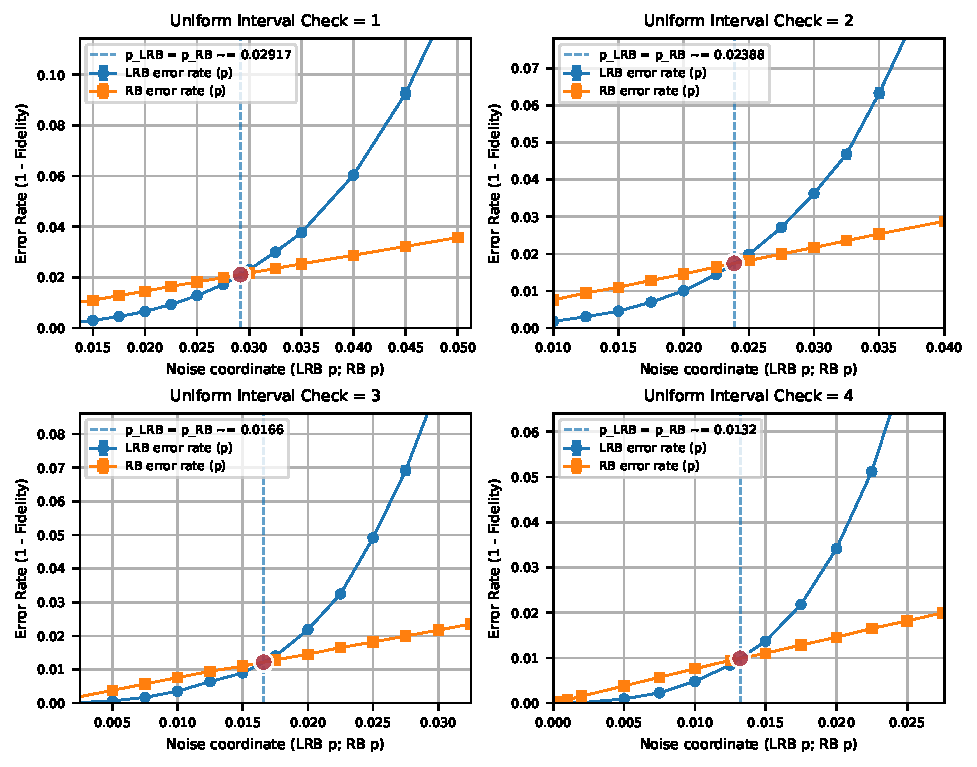
\includegraphics[width=0.75\textwidth]{figures/sdim140/si1000-1anc-threshold-grid.pdf}
  \caption{Fitted error rates per unit of depth of LRB-D (blue) and of the baseline, physical RB (orange), versus the two-qutrit gate error probability $p$ under SI1000 in the one-ancilla layout, for the intervals $k = 1$ to $4$, with central 68\% intervals of the parametric bootstrap; intervals that are not visible are smaller than the markers. Each panel shows a window around $p^\star(k)$ of the grid that merges the two runs: points at $p < 0.015$ come from the production run and points at $p \ge 0.015$ from the high-$p$ extension run, and the $k = 1$ panel shows only the latter. The panel titles give the interval $k$, the horizontal axis is $p$ for both curves, ``LRB'' and ``RB'' in the legends stand for LRB-D and the baseline, ``Error Rate (1 - Fidelity)'' is the error rate per unit of depth, and the first legend entry gives $p^\star(k)$. The vertical line and the large marker of each panel give the pseudo-threshold $p^\star(k)$ of \autoref{tab:pseudo_thresholds}.}
  \label{fig:threshold_grid_si1000_1anc}
\end{figure*}

% checks P-kdep-* (fits_all_k.csv, raw_per_depth.csv); full set: generated table kdep
Because all intervals of a production run share one set of circuits and shots (\autoref{sub:lrb_d}), a change of $k$ at fixed $p$ changes only which shots are accepted. Postselecting fewer rounds accepts more shots and raises $r_{\mathrm{LRB}}$ (\autoref{tab:kdep}, for $p = 5\times10^{-3}$ and $10^{-2}$; \autoref{fig:unif2_si1000_1anc} to \autoref{fig:unif4_sd6_1anc} show the traces). Under SI1000 at $p = 5\times10^{-3}$, the rejected fraction at $m = 10$ falls from its value at $k = 1$ (\autoref{sub:interval_results}) to 93.7\% at $k = 4$, while $r_{\mathrm{LRB}}$ rises by a factor of 4.1; under SD6 at the same $p$ the factor is 3.8. The rise is consistent with the pairs of faults of \autoref{sub:terminal_results}, which a round outside the postselection no longer separates: for $k = 2$ to $4$, $r_{\mathrm{LRB}}$ still grows as $p^{2.0}$ to $p^{2.1}$ between $p = 5\times10^{-4}$ and $2\times10^{-3}$. The fall of the pseudo-threshold with $k$ thus comes from $r_{\mathrm{LRB}}$ alone, because the baseline does not depend on $k$.

% checks P-model-* (canonical files), P-lrb-model, P-rb-model (fits_all_k.csv, p = 0.01, k = 1); full set: generated table model_ratio
In the one-ancilla layout the SD6 pseudo-thresholds exceed the SI1000 ones at every interval, by 9 to 37\%, which is 1.9 to 6.5 standard errors of their ratio (\autoref{tab:model_ratio}). At $p = 10^{-2}$ and $k = 1$, $r_{\mathrm{LRB}}$ is 5.2 times as large under SD6 as under SI1000, so the higher SD6 values do not come from a lower logical error rate (\autoref{tab:kdep} gives the other intervals). The baseline, whose gates fail with probability $p$ under SD6 and $p/10$ under SI1000 (\autoref{tab:circuit-noise}), has an error rate 10 times as large; the SD6 pseudo-thresholds are higher because the baseline grows by more than the logical error rate.

% checks P-acc-min, P-chi-* (merged tables: lrb_chi2/(lrb_n_points - 2), p = 0.015 to 0.035); brackets: generated table brackets
Two limits apply near the pseudo-thresholds. First, many of the fits that bracket them have few depths, and some have few accepted shots at their largest depth (\autoref{tab:brackets}). Eleven of the sixteen values of \autoref{tab:pseudo_thresholds}, among them all eight with $k \le 2$, rest on the depths $m \le 6$ alone, and under SD6 the fits that bracket $p^\star(1)$ and $p^\star(2)$ have three to five depths. Seven of the 32 bracketing fits, all for $k = 1$ or $4$, have fewer than ten accepted shots per sequence at their largest depth, down to $3.6$. With so few shots the modulus of the estimate is biased upward (\appref{app:campaign-fits}), which acts to lower the fitted $r_{\mathrm{LRB}}$ and to raise $p^\star$; the standard errors do not include this bias. Second, as under SD6 already for $k = 1$ (\autoref{sub:interval_results}), a single exponential is approximate near the SI1000 pseudo-thresholds for $k = 3$ and $4$; for $k \le 2$ it describes the decays closely. Under SI1000 between $p = 0.015$ and $0.035$, in both layouts, $\chi^2$ per degree of freedom is $0.1$ to $1.1$ for $k = 1$ and $2$, which is 4 to 33 times the value $1/N_s$ of \autoref{sub:fit_model}, and $1.3$ to $9.6$ for $k = 3$ and $4$, where the traces step at depths that are not multiples of $k$ (\appref{app:campaign-search}). The bracketing fits at $p < 0.015$, for $k = 4$ and for $k = 3$ in the two-ancilla layout, lie in the same range (\autoref{tab:brackets_rates}). Under SI1000, for $k = 3$ and $4$ the extension and the production fit at the same $p$, which hold different depths, differ by up to 16\% in $r_{\mathrm{LRB}}$ (\appref{app:campaign-runs}).

% checks P-step-min, P-order (sequence-bootstrap replicate files; full set: generated table fall_factors)
Within these limits, each of the sixteen entries of \autoref{tab:pseudo_thresholds} lies between two neighboring grid points at which $r_{\mathrm{LRB}}$ is below and above $r_{\mathrm{RB}}$, and for each of the sixteen the difference of the two changes sign nowhere else on its grid of $p$ (\autoref{tab:brackets}, \autoref{tab:brackets_rates}). Every step between adjacent intervals amounts to at least 6 standard errors when the bootstrap replicates are paired over the sequences that the intervals share, and the ordering $p^\star(1) > p^\star(2) > p^\star(3) > p^\star(4)$ holds in all 1000 replicates of every layout and noise model (\autoref{tab:fall_factors}).

\subsection{Two-Ancilla Layout}
\label{sub:layout_comparison}

% Layout gaps 1 - p*(two)/p*(one), relative standard errors in quadrature: generated table pstar; checks L-*
% Rejected fractions and fitted errors: raw_per_depth.csv, fits_all_k.csv (configs conv-*)
The longer check round of the two-ancilla layout lowers every pseudo-threshold, by 9 to 18\% under SI1000 and by 21 to 33\% under SD6 (\autoref{tab:pseudo_thresholds}). Each of these eight gaps between the layouts is 3.9 to 15.8 times its standard error. Because these standard errors include the choice of the baseline sequences (\autoref{sub:fit_model}), they account for the differences between the baseline error rates of the runs of the two layouts, which reach 9\% (\autoref{tab:rb_layouts}).

At equal $p$ and $k = 1$, the two-ancilla layout rejects more shots wherever shots are accepted, and its fitted $r_{\mathrm{LRB}}$ is the larger one at each of the ten grid points from $p = 5\times10^{-4}$ to $0.03$ (\autoref{fig:four_configs}; \autoref{fig:unif1_si1000_2anc} to \autoref{fig:threshold_grid_sd6_2anc}). Under SI1000 the two error rates differ by 0.8 to 4.1 standard deviations of the parametric bootstrap of their ratio over the ten grid points; $r_{\mathrm{LRB}}$ is larger by 16\% at $p = 5\times10^{-3}$ and by 12\% at $10^{-2}$ (2.0 and 2.1 standard deviations). Under SD6 it is larger by 56\% and 78\% at these two $p$ (9.1 and 8.6 standard deviations). At $p = 5\times10^{-3}$ a single round, at $m = 0$, rejects $24.8\%$ of the shots under SI1000 and $28.5\%$ under SD6, $2.7$ and $8.5$ percentage points more than in the one-ancilla layout (\autoref{tab:m0}).

\begin{figure*}[tp]
  \centering
  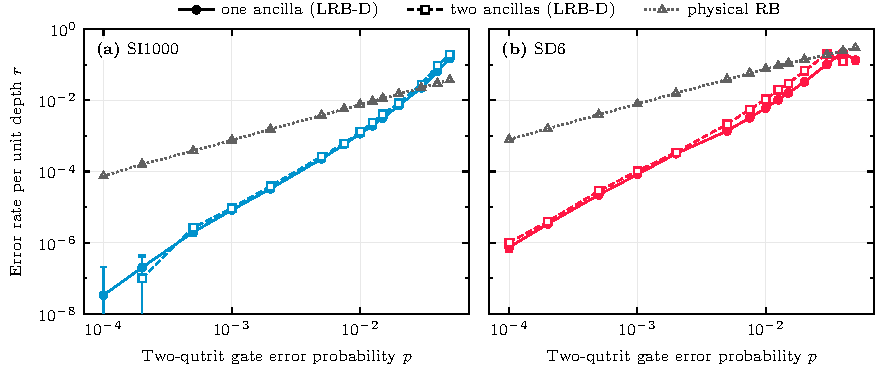
\includegraphics{figures/sdim140/lrb-vs-rb-k1.pdf}
  \caption{Fitted error rate per unit of depth for LRB-D with the postselection interval $k = 1$ versus the two-qutrit gate error probability $p$ under (a)~SI1000 and (b)~SD6, in the one-ancilla layout (filled circles, solid lines) and the two-ancilla layout (open squares, dashed lines), and for the baseline, physical RB under the same noise model, in the one-ancilla runs (open triangles, dotted lines). Error bars are central 68\% intervals of the parametric bootstrap; bars that are not visible are smaller than the markers, and intervals that reach zero run to the bottom of the axis. All points are fits to the production runs. At $p \ge 0.03$ every LRB-D fit rests on two or three depths (\autoref{tab:k1_depths}); the downturns of the SD6 curves at the largest $p$ come from such fits, and fits that return zero error are not drawn. The pseudo-thresholds of \autoref{tab:pseudo_thresholds} use the high-$p$ extension runs from $p = 0.015$ (SI1000) and $0.025$ (SD6) on, so they cannot be read off the crossings drawn here.}
  \label{fig:four_configs}
\end{figure*}

% Fault counts per round: Sec. 2.5 (67.9p, 76.3p, 73p, 103p; hw checks/check_fault_budgets.py); idle locations: scratch/writer-conv/budget.out; checks L-budget-*, L-gapdiff-*, L-rb-max
The gap is larger under SD6 at every interval, by 9 to 20 percentage points, which is 2.7 standard errors at $k = 2$ and 3.6 to 5.8 at the other intervals (\autoref{tab:model_ratio}). The fault counts go the same way: the data relay raises the expected number of faults per round by $8.4p$ under SI1000 and by $30p$ under SD6 (\autoref{sub:noise_models}), and under SD6 $22p$ of the $30p$ come from the 22 additional idle locations of the four extra gate moments, which SI1000 charges at $p/10$ (\appref{app:rounds-budget}).

% checks L-model-max, L-lrb-model, L-rb-model (fits_all_k.csv, configs conv-*, p = 0.01, k = 1)
With the larger gap under SD6, the two noise models give pseudo-thresholds within about 10\% of each other in the two-ancilla layout, at most 3.3 standard errors apart (\autoref{tab:model_ratio}). From SI1000 to SD6, $r_{\mathrm{LRB}}$ at $p = 10^{-2}$ and $k = 1$ now grows by a factor of 8.3, close to the factor of 9.5 by which the baseline of the same runs grows.

\subsection{Comparison with the Qubit Code}
\label{sub:qubit_comparison}

% Qubit p* and seq_boot_se: comparisons/pseudo-thresholds-qubit-current.csv (qubit-one-ancilla rows only) and pseudo-thresholds-qubit-conv-sites-current.csv; table body: generated table qubit; checks Q-*
For the qubit $[[5,1,2]]$ code every pseudo-threshold lies below that of the qutrit code in the same layout, under the same noise model and at the same interval (\autoref{tab:pseudo_thresholds_qubit}, \autoref{fig:pstar_qubit_qutrit}). The ratio $p^\star_{\mathrm{qubit}}/p^\star_{\mathrm{qutrit}}$ is 0.29 to 0.38 under SI1000 and 0.45 to 0.56 under SD6, and each of the sixteen ratios lies more than 15 standard errors below one. On the qutrit grids the tolerance and the error floor that the qubit search omits (\autoref{sub:qubit_code}, \appref{app:campaign-search}) change none of the sixteen values of \autoref{tab:pseudo_thresholds}, so each ratio compares two crossings located by the same search rule. Both limits of \autoref{sub:pseudo_thresholds} apply to the qubit values as well. Three of their 32 bracketing fits, all under SD6, have fewer than ten accepted shots per sequence at their largest depth; the fits that bracket $p^\star(1)$ and $p^\star(2)$ under SD6 again have three to five depths, and those under SI1000 have six or nine. $\chi^2$ per degree of freedom of the bracketing fits is $0.01$ to $0.5$ for $k \le 2$ and $0.7$ to $2.3$ for $k = 3$ and $4$ (\autoref{tab:brackets_qubit}, \autoref{tab:brackets_rates_qubit}). Within these limits, all sixteen qubit values are crossings between two neighboring points of the refinement runs.

\begin{table*}[tp]
  \centering
  \begin{tabular}{cc|cc|cc}
    \hline
    & & \multicolumn{2}{c|}{SI1000} & \multicolumn{2}{c}{SD6} \\
    layout & $k$ & $p^\star_{\mathrm{qubit}}$ & $p^\star_{\mathrm{qubit}}/p^\star_{\mathrm{qutrit}}$ & $p^\star_{\mathrm{qubit}}$ & $p^\star_{\mathrm{qubit}}/p^\star_{\mathrm{qutrit}}$ \\
    \hline
    % BEGIN GEN qubit
    one-ancilla & 1 & $0.0112 \pm 0.0002$ & $0.38 \pm 0.01$ & $0.0210 \pm 0.0008$ & $0.53 \pm 0.03$ \\
     & 2 & $0.0078 \pm 0.0002$ & $0.33 \pm 0.01$ & $0.0151 \pm 0.0005$ & $0.56 \pm 0.02$ \\
     & 3 & $0.00495 \pm 0.00009$ & $0.30 \pm 0.01$ & $0.0094 \pm 0.0003$ & $0.52 \pm 0.02$ \\
     & 4 & $0.00395 \pm 0.00008$ & $0.30 \pm 0.01$ & $0.0072 \pm 0.0002$ & $0.47 \pm 0.02$ \\
    \hline
    two-ancilla & 1 & $0.0093 \pm 0.0001$ & $0.35 \pm 0.01$ & $0.0142 \pm 0.0004$ & $0.50 \pm 0.02$ \\
     & 2 & $0.0064 \pm 0.0001$ & $0.31 \pm 0.01$ & $0.0100 \pm 0.0003$ & $0.47 \pm 0.01$ \\
     & 3 & $0.00395 \pm 0.00008$ & $0.29 \pm 0.01$ & $0.0061 \pm 0.0002$ & $0.50 \pm 0.02$ \\
     & 4 & $0.00313 \pm 0.00005$ & $0.29 \pm 0.01$ & $0.0047 \pm 0.0001$ & $0.45 \pm 0.01$ \\
    % END GEN qubit
    \hline
  \end{tabular}
  \caption{Pseudo-thresholds $p^\star(k)$ of the qubit $[[5,1,2]]$ code against single-qubit RB under the same noise model at the same two-qubit gate error probability $p$, for the postselection intervals $k = 1$ to $4$, and their ratio to the qutrit values of \autoref{tab:pseudo_thresholds} for the same layout, noise model and interval. Uncertainties are one standard error (68\% confidence), from a bootstrap over the random Clifford sequences. The relative standard error of a ratio is the two relative standard errors added in quadrature (\appref{app:campaign-bootstrap}).}
  \label{tab:pseudo_thresholds_qubit}
\end{table*}

\begin{figure*}[tp]
  \centering
  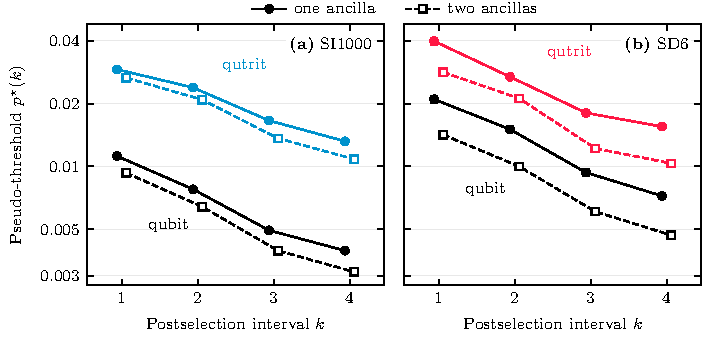
\includegraphics{figures/sdim140/pstar-qubit-vs-qutrit.pdf}
  \caption{Pseudo-threshold $p^\star(k)$ versus the postselection interval $k$ for the $[[5,1,2]]_3$ code (qutrit; blue in (a), red in (b)) and the qubit $[[5,1,2]]$ code (black) under (a)~SI1000 and (b)~SD6, in the one-ancilla layout (filled circles, solid lines) and the two-ancilla layout (open squares, dashed lines). Each $p^\star$ is the crossing of the LRB-D error rate with the error rate of physical RB of the same local dimension under the same noise model. Error bars are one standard error (68\% confidence) from the bootstrap over the random Clifford sequences; bars that are not visible are smaller than the markers. For legibility the two layouts are drawn $0.06$ to the left and right of each $k$, and the lines guide the eye.}
  \label{fig:pstar_qubit_qutrit}
\end{figure*}

% checks Q-fall-*, Q-gap-* (canonical files, replicate files); full sets: generated tables fall_factors, qubit_layout_gap
The qubit pseudo-thresholds depend on the interval and on the layout in the same directions as the qutrit ones. They fall with $k$ in all 1000 replicates of every layout and noise model, by factors of 2.8 to 3.0 from $k = 1$ to $4$. Each factor is 1.1 to 1.3 times the qutrit factor of the same layout and noise model, a difference of 7.0 and 8.6 standard errors of their ratio under SI1000 and of 2.2 and 2.9 under SD6 (\autoref{tab:fall_factors}). The two-ancilla layout lowers them by 17 to 21\% under SI1000 and by 32 to 35\% under SD6, which is 7.9 to 12.6 standard errors (\autoref{tab:qubit_layout_gap}).

% checks Q-rb-*, Q-est-* (refits of the production runs; word lengths from the RB circuits); full set: generated table rb_ratio
Of the two error rates that cross at a pseudo-threshold, the baseline error rate is smaller for the qubit code at equal $p$. In the production runs of both layouts, at every $p > 0$ of the grid, the qubit $r_{\mathrm{RB}}$ is 0.44 to 0.48 times the qutrit one under SI1000 and 0.42 to 0.49 times under SD6 (\autoref{tab:rb_ratio}; \autoref{fig:k1_qubit_qutrit} shows the one-ancilla layout; \appref{app:campaign-fits} gives the factor that converts these ratios to $1 - f$). The error added per gate and the number of gates per Clifford account for this ratio. To first order in its probability $p_1$, the DEP1 channel after a primitive gate adds $q\,p_1/(q+1)$ to the error rate, that is, $2p_1/3$ for a qubit and $3p_1/4$ for a qutrit. With the mean numbers of primitive gates per Clifford of \autoref{sub:qubit_code} and \autoref{sub:fit_model}, these give a ratio of $8/9$ times the ratio of the two means, 0.44. With the numbers drawn in the qubit and the qutrit run of each layout and noise model, the estimate stays within 0.02 of the fitted ratio of these two runs for every $p \le 10^{-2}$ (\autoref{tab:rb_ratio}; \appref{app:campaign-data} extends the estimate to larger $p$).

\begin{figure*}[tp]
  \centering
  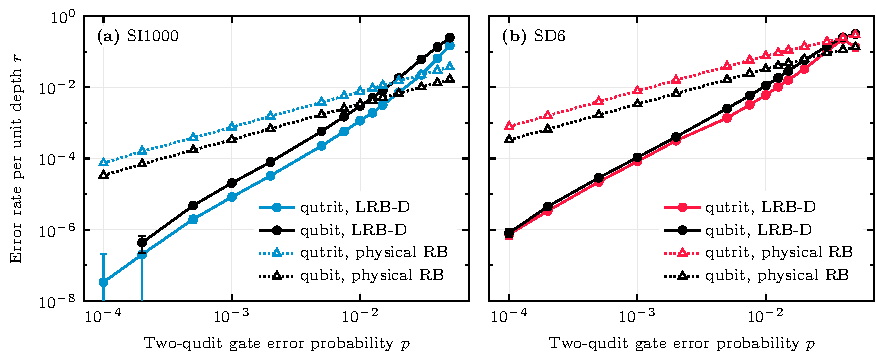
\includegraphics{figures/sdim140/lrb-vs-rb-k1-qubit-vs-qutrit.pdf}
  \caption{Fitted error rate per unit of depth versus the two-qudit gate error probability $p$ for the $[[5,1,2]]_3$ code (qutrit; blue in (a), red in (b)) and the qubit $[[5,1,2]]$ code (black) in the one-ancilla layout under (a)~SI1000 and (b)~SD6: LRB-D with the postselection interval $k = 1$ (filled markers, solid lines) and the baseline, physical RB of the same local dimension (open triangles, dotted lines). The error rate is $r = (q-1)(1-f)/q$ for local dimension $q$ and decay parameter $f$. Error bars are central 68\% intervals of the parametric bootstrap; bars that are not visible are smaller than the markers, and intervals that reach zero run to the bottom of the axis. All points are fits to the production runs. At $p \ge 0.03$ every LRB-D fit rests on two or three depths. The qubit LRB-D fit at $p = 10^{-4}$ under SI1000 returns zero error and is not drawn.}
  \label{fig:k1_qubit_qutrit}
\end{figure*}

% checks Q-lrb-*, Q-ex-*, Q-rej-*, Q-gates-* (refits of the production runs; scratch/writer-qubit/analysis.out X6); full set: generated table lrb_ratio
The logical error rate, in contrast, is larger for the qubit code. In both layouts, under both noise models and for $k = 1$ to $4$, the qubit $r_{\mathrm{LRB}}$ exceeds the qutrit one at every grid point of the production runs from $p = 10^{-3}$ up to the qutrit pseudo-threshold, by more than three standard deviations of the parametric bootstrap of their ratio. Between $p = 10^{-3}$ and $10^{-2}$ it is 2.4 to 3.0 times as large under SI1000 and 1.3 to 2.1 times under SD6 (\autoref{tab:lrb_ratio}; \autoref{fig:k1_qubit_qutrit} shows $k = 1$ in the one-ancilla layout). These error rates describe a larger fraction of the shots, since the qutrit code rejects more wherever both codes accept any: under SI1000 at $p = 5\times10^{-3}$ and $k = 1$ the qubit code rejects 60\% of the shots at $m = 2$ and 97\% at $m = 10$ (\autoref{tab:rej_qubit}; \autoref{sub:interval_results} gives the qutrit values). The mechanism behind the larger qubit logical error rate is open. With the same expected number of faults in a check round and about half as many in a logical Clifford as the qutrit code (\autoref{sub:noise_models}, \autoref{sub:qubit_code}), the qubit circuits hold fewer expected faults at equal $p$, so the number of faults does not explain it. The lower qubit pseudo-thresholds thus combine both differences: a smaller baseline error rate and a larger logical error rate each move the crossing to smaller $p$.
